\section{Probability}

\subsection{Basics}

\subsubsection{Probability space}

Probability works on some basic entites:
\begin{itemize}
    \item \samplespace is a nonempty set called the samplespace. 
    \item $\omega \in \samplespace$ is called an outcome
    \item $E \subseteq \samplespace$ is called an event
\end{itemize}


\begin{definition}[Probability]
    Probability is a measure on \samplespace. It is a total function $ \probFunct: \samplespace \to \reals $ such that:
    \begin{itemize}
        \item $ \forall \omega \in \samplespace : \probFunct[\omega] \geq 0 $
        \item $ \sum_{\omega \in \samplespace} \probFunct[\omega] = 1 $
    \end{itemize}
\end{definition}

A probability measure together with a samplespace is called a probability space. 


We define the probability of an event as: 
$$ \probFunct[E] = \sum_{\omega \in E} \probFunct[\omega] $$

\begin{definition}[Random variable]
    A random variable is a function mapping a $\omega$ from \samplespace  to the reals. 
    $$ X(\omega) : \samplespace \then \reals $$
\end{definition}
Note that a random variable strictly takes a single $\omega$ as argument, not a set of outcomes. 

We then calculate the probability that a random variable $X$ has a certain value $x$ as such: 

$$ \probFunct[X=x] = \sum_{X^{-1}(x)} \probFunct[\omega] $$

\begin{definition}[Expectation]
    The expectation of a random variable is defined as 
    $$ E[X] = \sum_\samplespace X(\omega)P(\omega)$$ 
\end{definition}

\begin{definition}[Conditional Probability]
    $$ \probFunct[A | B] = \frac{\probFunct[A \intersection B]}{\probFunct[B]}$$
\end{definition}

As a nice little exercise, we prove the formula for the conditional probability of the \emph{complement} of $B$.

\begin{proof}
    $$ \probFunct[A | \overline{B}] = $$
\end{proof}



As an illustrative example, consider the following probabilities. People can be \emph{small} (S) or \emph{tall} (T). They can be \emph{good} (G) or \emph{bad} (B) at basketball.
Here are the tables of probabilities:

\begin{table}[H]
    \centering
    \begin{tabular}{llllll}
      &      &  &   & S    & T    \\
      &      &  &   & 0.6  & 0.4  \\
      &      &  &   &      &      \\
      &      &  &   & S    & T    \\
    B & 0.14 &  & B & 0.54 & 0.08 \\
    G & 0.86 &  & G & 0.6  & 0.32
    \end{tabular}
\end{table}

\begin{table}[H]
    \centering
    \begin{tabular}{llll}
        $P(B|S)$ & 0.9 & $P(B|T)$ & 0.8 \\
        $P(G|S)$ & 0.1 & $P(G|T)$ & 0.2 
    \end{tabular}
\end{table}

Notice the following facts:
\begin{itemize}
    \item notice how $P(G|T) \neq 1 - P(G|S)$
    \item notice how $P(G|T) = 1 - P(B|T)$
    \item $P(A, B) = P(A|B) P(B) = P(B|A) P(A)$
    \item $ \Sigma_A \Sigma_B P(A, B) = 1.0 $
\end{itemize}

As yet another exercise, here is the formula of the probability of a union of arbitrary events: 

\begin{proof}
    $$ \probFunct (\union A_i) = \sum_i \probFunct(A_i) 
            - \sum_i \sum_{j>i} \probFunct(A_i \intersection A_j) 
            + \sum_i \sum_{j>i} \sum_{k>j} \probFunct(A_i \intersection A_j \intersection A_k) 
            - ...  $$
    
    This is proven by induction. 
                
    \subprf{Base case:}{$\probFunct(A_1 \union A_2) = \probFunct(A_1) + \probFunct(A_2) - \probFunct(A_1 \intersection A_2) $}{
        This is tirivally true when looking at a Venn Diagramm. 
    }
    \subprf{Induction step. Suppose that... }{ }{
    }
    
    
\end{proof}

\subsubsection{A few lemmas on conditional probability} \label{condPropLemmas}

In a "causal" chain of events $A, B, C$ we can integrate out the middle-event $B$.
\begin{equation}
    \begin{aligned}
        p(A, B, C)  &= \frac{p(A, B, C)}{p(A, B)} \frac{p(A, B)}{p(A)} p(A) \\
                    &= p(C|AB) p(B|A) p(A) \\
    \end{aligned}
\end{equation}

\begin{equation}
    p(A, C) = \Sigma_B p(A, B, C)
\end{equation}

\begin{equation}
    \begin{aligned}
            p(C | A) &= \frac{p(A, C)}{p(A)} \\
                     &= \Sigma_B p(C|A, B) p(B|A)
    \end{aligned}
\end{equation}

We can take the expression for conditional probability and condition \emph{every term} on a third event.
\begin{equation}
    \begin{aligned}
        p(B|A, C) &= \frac{p(A, B, C)}{p(A, C)} \\
        p(A|B, C) &= \frac{p(A, B, C)}{p(B, C)} \\
        p(A|B, C) &= \frac{p(B|A, C) p(A|C) p(C)}{p(B|C)p(C)} \\
                  &= \frac{p(B|A, C) p(A|C)}{p(B|C)} \\
    \end{aligned}
\end{equation}


\subsection{Decomposing variance - the road to sensitivity analysis}

\paragraph{Expressing variance as expectation} ...
\begin{equation}
    \begin{aligned}
        V_X &= E_{ (X - E_X)^2 } \\
            &= E_{ X^2 - 2 X E_X + E_X^2 } \\
            &= E_{X^2} - E_X^2
    \end{aligned}
\end{equation}

\paragraph{Conditional expectation and variance} ...

\begin{definition} \label{conditionalExpectation}
    Conditional expectation:
    $$ E_{Y|x} = \Sigma y P(y|x) $$
\end{definition}

\begin{definition} \label{conditionalVariance}
    Conditional variance: 
    $$ V_{Y|x} = E_{(Y - E_{Y|x})^2 | x} $$ 
\end{definition}

\paragraph{Law of total expectation} ...
\begin{equation} \label{lawOfTotalExpectation}
    \begin{aligned}
        E_Y &= \Sigma_Y y P(y) \\
            &= \Sigma_Y y \Sigma_X P(y|x) P(x) \\
            &= \Sigma_X (\Sigma_Y y P(y|x)) P(x) \\
            &= \Sigma_X E_{Y|x} P(x) \\
            &= E_{E_{Y|x}}
    \end{aligned}
\end{equation}

\paragraph{Law of total variance} ...
\begin{equation} \label{lawOfTotalVariance}
    \begin{aligned}
        V_Y &= E_{Y^2} - E_Y^2 \\
            &= E_{E_{Y^2 | X}} - E^2_{E_{Y|X}} \\
            &= E_{  V_{Y|X} + E^2_{Y|X}  } - E^2_{E_{Y|X}} \\
            &= E_{V_{Y|X}} + E_{E^2_{Y|X}} - E^2_{E_{Y|X}} \\
            &= E_{V_{Y|X}} + V_{E_{Y|X}}
    \end{aligned}
\end{equation}


\begin{figure}[h]
    \caption{Illustration of the law of total variance}
    \centering
      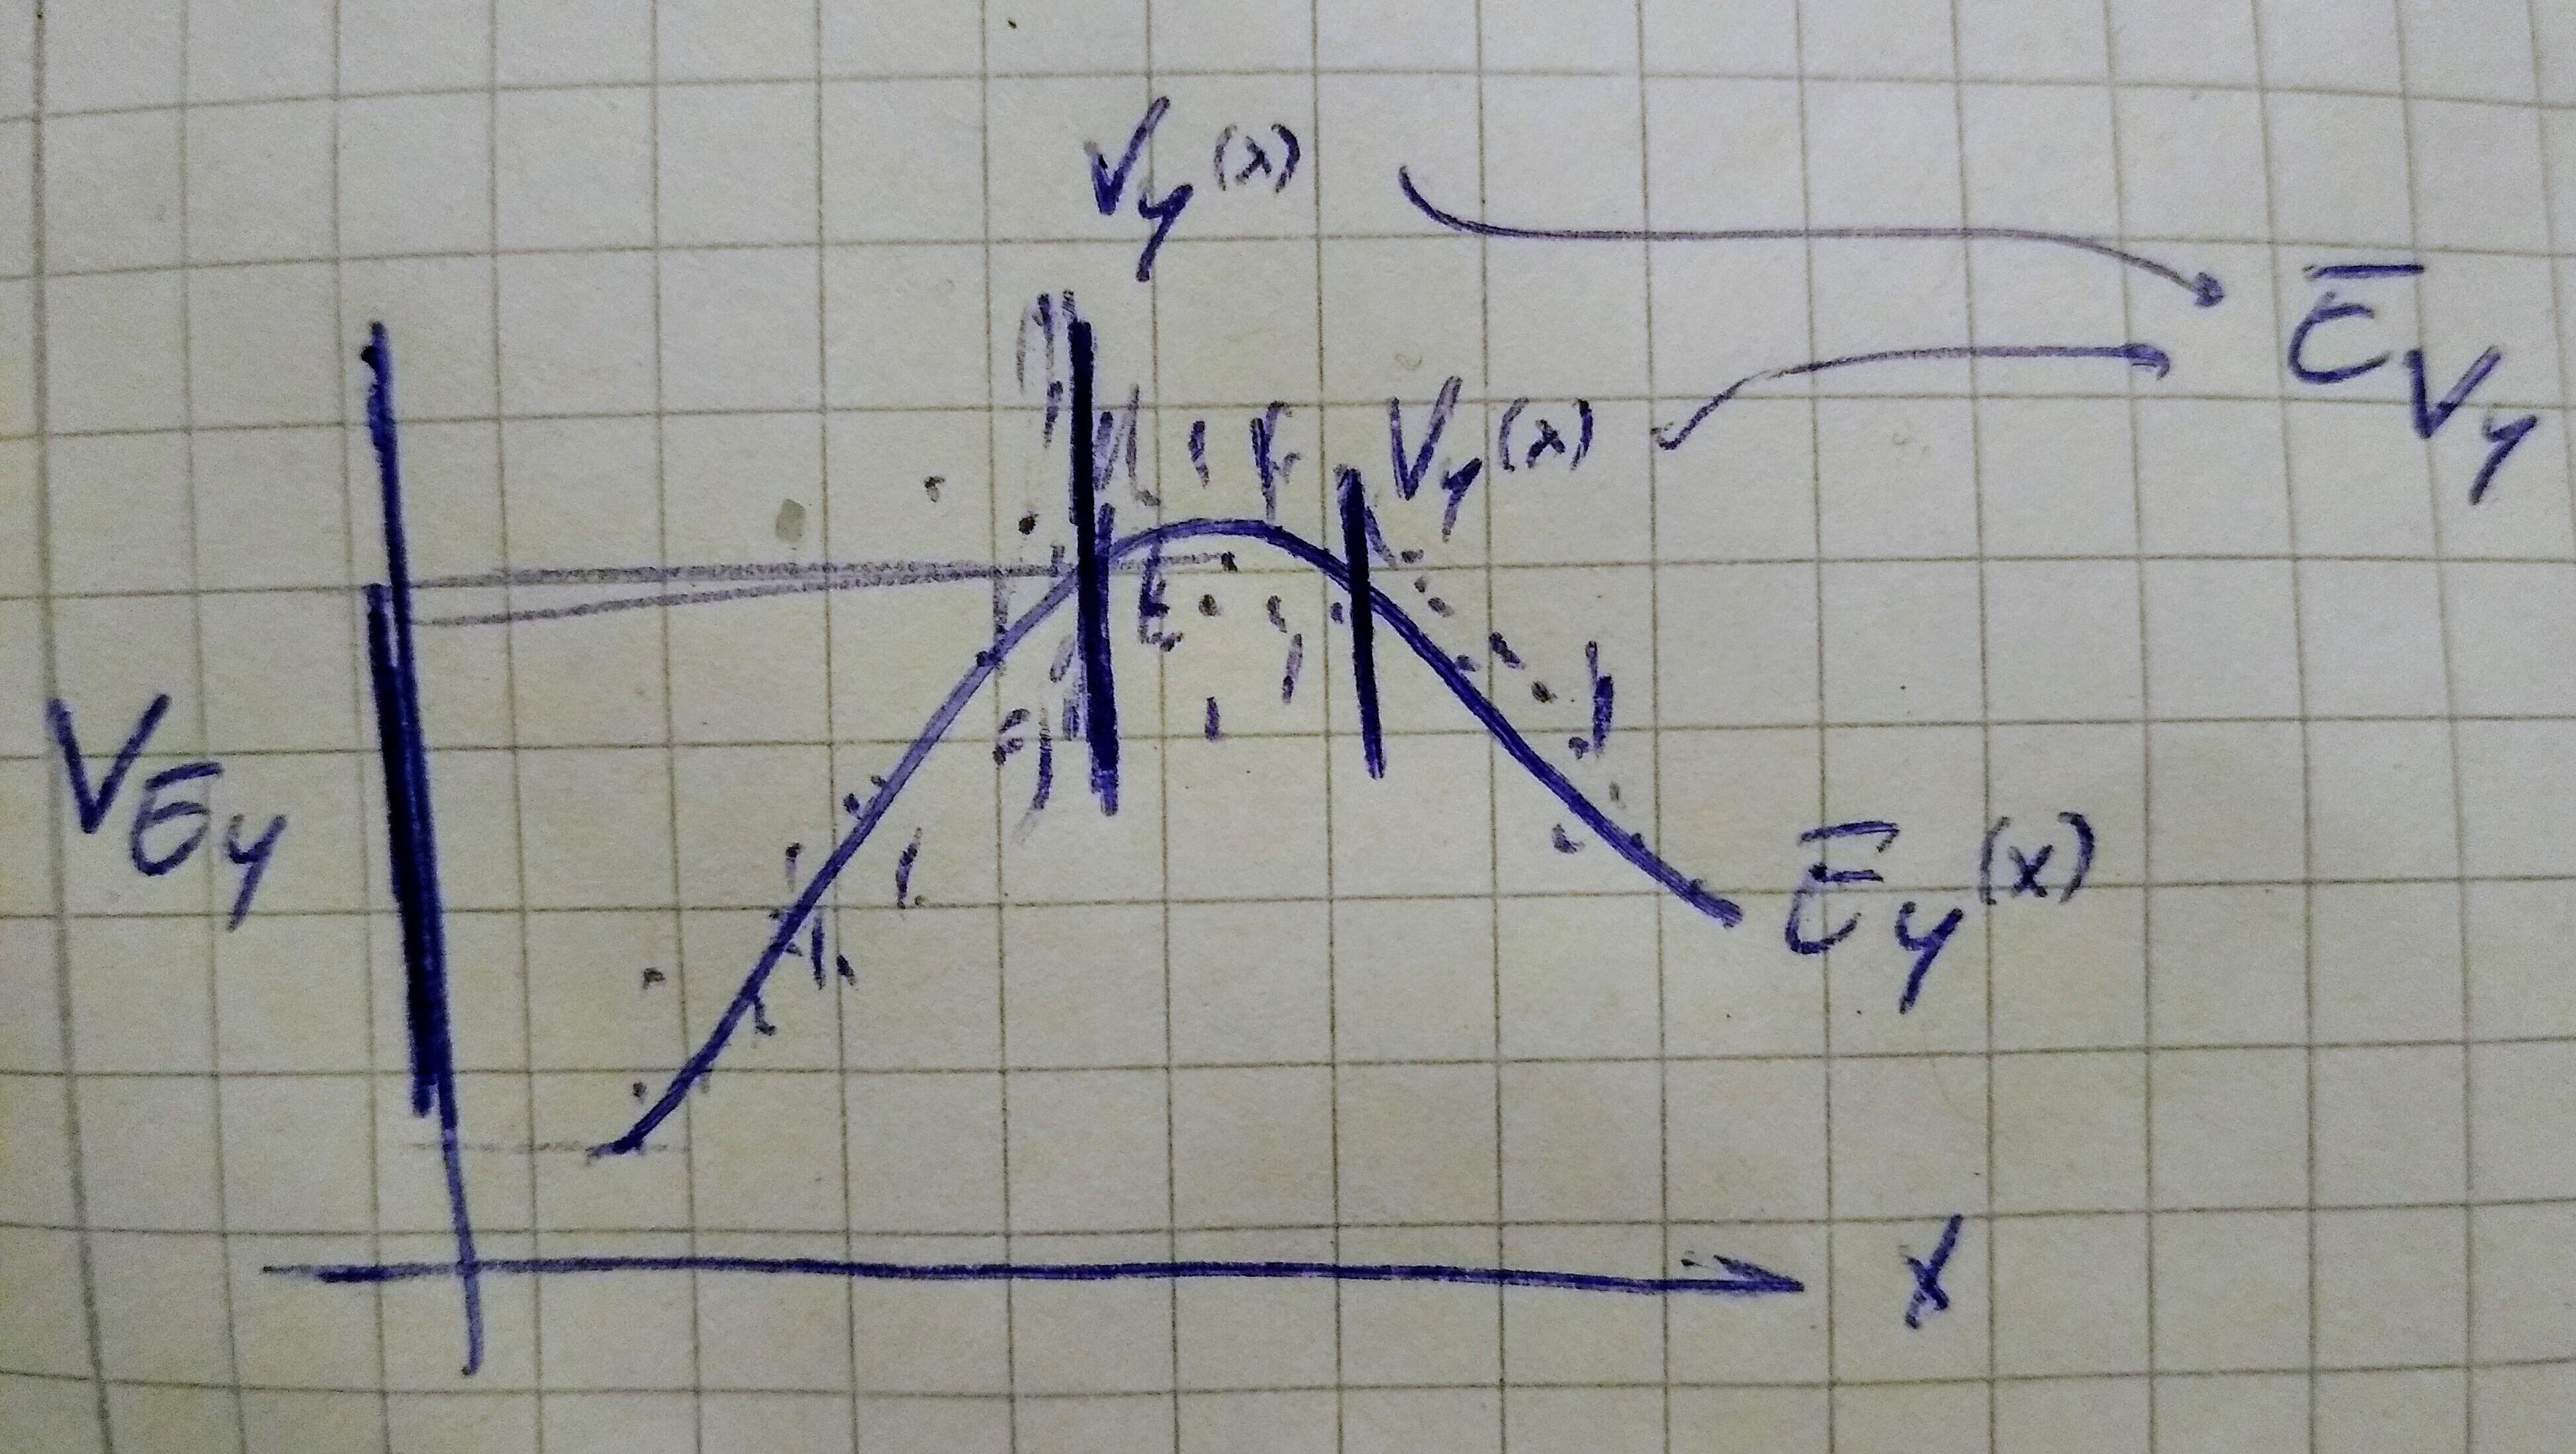
\includegraphics[width=0.5\textwidth]{images/law_of_total_variance.jpg}
\end{figure}
 
 
\subsection{Probability density functions}
Up to now we have been dealing with probability mass functions on discrete variables.
That works just as well with discrete variables, but we need to accommodate some details.
For example, we can only define probability density in therms of cumulative probability functions.

Let $P(x) := Pr(X > x)$ be a cumulative probability function.
Then the probability density at $x$ is $\frac{d P}{d x}(x)$.

\paragraph{As an exercise,} consider $x \tilde Exp(x)$. We want to calculate $E(x | x > x_0)$. 
We'll start with $P(x | x > x_0)$.
We have:
\begin{equation}
    \begin{aligned}
        P(X | X > x_0) &= \left( \text{ using the fact that } P(B|A) = \frac{P(A \land B)}{P(A)} \right) \\
                          &= \frac{ P(X = x \land X > x_0) }{ P(X > x_0) } \\
                          &= \frac{ s_{x_0} P(X=x) }{ P(x > x_0) }  (\text{ with $s_{x_0}$ the step-function at $x_0$}) \\
                          &= \frac{ s_{x_0} P(X=x) }{ \int_{x_0}^\infty p(x) dx }
    \end{aligned}
\end{equation}

This leads us to the expectation:

\begin{equation}
    \begin{aligned}
        E(X | X > x_0)  &= \int_{-\infty}^\infty x p(X | X > x_0) dx \\
                        &= \frac{ s_{x_0} \int_{-\infty}^\infty x p(x) dx }{ \int_{x_0}^\infty p(x) dx } \\
                        &= \frac{ \int_{x_0}^\infty x p(x) dx }{ \int_{x_0}^\infty p(x) dx } \\
                        &= \frac{ s_{x_0} E(X) }{ P(X > x_0) } 
    \end{aligned}
\end{equation}


\subsection{Probability distributions}

A probability distribution is a function from the domain of a random variable to its probability - in other words, a probability distribution yields the probability that a random variable will take on a certain value. 

There is an abundance of ready made probability distributions to chose from, covering virtually all important situations. But care must be taken when deciding which distribution to apply to a certain problem. 

\paragraph{The Bernoulli family} based on modelling a series of coin-tosses.
\begin{itemize}
    \item Bernoulli: heads or tails?
    \item Binominal: k heads in n trials
    \item Poisson: k heads in $\infty$ trials. 
\end{itemize}
A remarkable feature of the Poisson-distribution is that it has only a parameter for the mean, but always the same variance.

\paragraph{The geometric family} based on repeating an experiment until it succeeds. 



\subsubsection{Probabilistic fallacies}
\begin{itemize}
    \item T-Test interpretation: If $\probFunct[A|B] = x$, then this does \emph{not} mean that $\probFunct[A|\overline{B}] = 1 - x$.
    \item Prosecutors fallacy aka. inverse fallacy: $P(A|B) \neq P(B|A)$
\end{itemize}

\paragraph{$\probFunct[A|\overline{B}] \neq 1 - \probFunct[A | B]$}. 
\begin{proof}
    By contradiction. 
    \begin{equation}
        \begin{aligned}
           \probFunct[A|B]                 &= 1 - \probFunct[A | \overline{B}] \\
                                           &= \frac{  \probFunct[B] - \probFunct[A \intersection \overline{B}]  }{  \probFunct[B]  }  \\
           \probFunct[A|B] \probFunct[B]   &=         \probFunct[B] - \probFunct[A \intersection \overline{B}] \\
           \probFunct[A \intersection B]   &= \probFunct[B] - \probFunct[A \intersection \overline{B}] \\
           \probFunct[A \intersection B] + \probFunct[A \intersection \overline{B}]  &= \probFunct[B] \\
           \probFunct[A] &= \probFunct[B]
        \end{aligned}
    \end{equation}
    Thus $\probFunct[A|\overline{B}] \neq 1 - \probFunct[A | B]$. But not that it \emph{does} hold true that $\probFunct[\overline{A}|B] = 1 - \probFunct[A | B]$
\end{proof}

